% La perception n'est pas la causalité -- version française du préprint.
% Compile avec pdflatex + bibtex, ou avec tectonic. Les figures sont dans
% paper/figures/ (régénérer les tracés via paper/make_figures.py).
\documentclass[11pt]{article}

\usepackage[utf8]{inputenc}
\usepackage[T1]{fontenc}
\usepackage[french]{babel}
\usepackage[margin=1in]{geometry}
\usepackage{amsmath,amssymb}
\usepackage{graphicx}
\usepackage{booktabs}
\usepackage{xcolor}
\usepackage[numbers,sort&compress]{natbib}
\usepackage[hidelinks]{hyperref}

\newcommand{\succf}{\mathrm{succ}}

\title{La perception n'est pas la causalité :\\
auditer les apprenants de représentations face à une vérité-terrain
causale exacte}
\author{Zaccarie Aglas\\ Chercheur indépendant\\ \texttt{zaccarie@zaccarie.fr}}
\date{\today}

\begin{document}
\maketitle

\begin{abstract}
L'apprentissage de représentations est généralement évalué sans accès à la
structure causale des données : une sonde atteint 85\,\% de précision et l'on
ne peut dire si une caractéristique est réellement représentée ou si le chiffre
est un artefact. Nous introduisons un banc d'essai où la structure causale est
connue \emph{exactement}. Sur des automates cellulaires élémentaires et des
réseaux booléens aléatoires assez petits pour être énumérés, toute la
dynamique --- bassins d'attraction, attracteurs, états garden-of-Eden, quotient
de bisimulation --- est calculée exactement et sert de vérité-terrain. Nous en
tirons quatre résultats. (i) Un modèle entraîné uniquement à prédire la
dynamique forward développe une représentation qui encode linéairement des
faits causaux \emph{locaux} (appartenance au garden-of-Eden, in-degré). (ii) Une
discrétisation compressée et préservant la structure de l'espace d'états
\emph{existe} prouvablement --- le quotient dynamique. (iii) Pourtant, cinq
objectifs de tokenisation appris standards --- reconstruction, prédiction
1-pas, prédiction multi-horizon, et deux variantes contrastives temporelles ---
échouent tous à la récupérer. Nous expliquons cet échec : le quotient dynamique
est \emph{perceptuellement éclaté}, aussi dispersé dans l'espace d'observation
qu'une partition aléatoire ; les objectifs biaisés vers la proximité
d'observation optimisent donc une géométrie orthogonale à la géométrie causale.
La barrière est structurelle, ce n'est pas un artefact d'optimisation. (iv) Cet
échec reste néanmoins propre à la classe d'objectifs : un objectif défini
récursivement sur la dynamique --- une métrique de bisimulation apprise ---
récupère le quotient (information mutuelle ajustée jusqu'à $0{,}95$), là où tout
objectif de proximité d'observation reste proche de zéro. Un seul biais inductif
--- la localité --- unifie le succès local et l'échec global.
\end{abstract}

\section{Introduction}

Les études de probing demandent si une représentation apprise encode une
propriété des données. Elles rapportent une précision. Mais sans la vraie
structure des données, cette précision est difficile à calibrer : elle confond
« la caractéristique est explicitement représentée » avec « une sonde
puissante peut la calculer » et avec des artefacts au niveau du hasard. Les
études de représentations du monde émergentes rencontrent le même fossé : la
vérité-terrain (par exemple un état de plateau) est connue, mais la structure
\emph{dynamique} (quels états sont causalement équivalents, lesquels sont
inatteignables, comment les trajectoires convergent) n'est pas énumérée.

Nous comblons ce fossé. Nous étudions des systèmes dynamiques discrets assez
petits pour être énumérés complètement. Pour un automate cellulaire élémentaire
sur $n$ cellules il y a $2^n$ états ; pour $n \le 20$ nous construisons le
graphe de transition d'états entier et en calculons, \emph{exactement et sans
échantillonnage}, tout objet dynamique d'intérêt : attracteurs, bassins
d'attraction, pré-images, états garden-of-Eden, longueurs de transitoire, et le
quotient de bisimulation. Cette vérité-terrain exacte permet d'auditer un
apprenant de représentations comme on audite un modèle face à une réponse
connue.

À partir du banc d'essai nous établissons quatre résultats.

\begin{itemize}
  \item \textbf{L'entraînement forward récupère la structure causale locale}
    (Section~\ref{sec:local}). Un modèle entraîné uniquement à prédire l'état
    suivant développe une représentation d'où des faits causaux \emph{locaux}
    --- appartenance au garden-of-Eden, in-degré --- sont décodables
    linéairement, bien au-dessus des baselines observation brute et réseau non
    entraîné. La structure long-horizon (appartenance à un bassin) n'est
    \emph{pas} récupérée.
  \item \textbf{La discrétisation préservant la structure existe}
    (Section~\ref{sec:exists}). Une tokenisation compressée qui préserve
    exactement la structure de bassins existe prouvablement : le quotient
    dynamique. Nous l'exhibons par construction.
  \item \textbf{Les tokeniseurs appris échouent à la récupérer}
    (Section~\ref{sec:fail}). Cinq objectifs de tokenisation appris standards
    échouent tous. La Section~\ref{sec:why} explique pourquoi : le quotient
    dynamique est \emph{perceptuellement éclaté}, si bien que les objectifs de
    proximité d'observation lui sont structurellement inadaptés.
  \item \textbf{Un objectif récursif la récupère}
    (Section~\ref{sec:positive}). Un objectif défini récursivement sur la
    dynamique --- une métrique de bisimulation apprise --- récupère le quotient
    que les objectifs perceptuels manquent, situant l'échec dans l'objectif et
    non dans les données.
\end{itemize}

Un seul mécanisme --- un biais inductif vers la localité dans l'espace
d'observation --- rend compte à la fois du résultat positif (la structure
locale est récupérée) et du négatif (le quotient non-local est manqué).

\section{Travaux connexes}
\label{sec:related}

\paragraph{Représentations du monde émergentes et probing.}
Sonder l'état latent d'un système sous-jacent à un modèle séquentiel est un
paradigme établi ; \citet{li2023emergent} entraînent un modèle séquentiel sur
une tâche synthétique et sondent l'état du monde. Les sondes linéaires
\citep{alain2016probes} opérationnalisent « explicitement représenté ». Nous
différons sur deux points : notre vérité-terrain est la structure
\emph{dynamique} entière (bassins, attracteurs, quotient de bisimulation),
exactement énumérée ; et notre objet d'étude central est l'\emph{échec}
systématique des tokeniseurs appris, avec une explication structurelle.

\paragraph{Bisimulation et abstraction d'états.}
Les métriques de bisimulation apprennent des représentations qui fusionnent les
états comportementalement équivalents \citep{zhang2021dbc,castro2021mico}. Notre
banc d'essai offre un cadre où le quotient de bisimulation est connu
exactement, de sorte que de telles méthodes peuvent être validées face à la
vérité-terrain plutôt qu'évaluées seulement par le retour aval.

\paragraph{World models, tokenisation, information.}
Les world models à latents discrets et tokenisés \citep{vandenoord2017vqvae,
hafner2023dreamerv3} motivent notre cadre de « tokeniseur appris ». Le goulot
d'information \citep{tishby1999ib} et la séparation par Shannon de la
transmission et du sens \citep{shannon1948} cadrent les questions de
compression.

\paragraph{Dynamique discrète.}
L'analyse exacte de l'espace d'états d'un automate cellulaire --- bassins
d'attraction, paramètre $Z$, bord du chaos --- suit \citet{wuensche1999z}.
L'analyse des réseaux récurrents comme systèmes dynamiques
\citep{sussillo2013blackbox} est un précédent méthodologique.

% À FAIRE : étoffer le positionnement vs Othello-GPT et la littérature
% contrastive \citep{vandenoord2018cpc}.

\section{Le banc d'essai : dynamique discrète à vérité-terrain exacte}
\label{sec:testbed}

\paragraph{Systèmes.}
Un automate cellulaire élémentaire (ECA) est un automate binaire
unidimensionnel à voisinage de rayon 1 et bord périodique ; une règle est l'une
des $256$ fonctions de mise à jour locales. Un état de $n$ cellules est un
entier de $[0, 2^n)$. Nous utilisons aussi des réseaux booléens aléatoires
(RBN) --- le modèle de Kauffman, à câblage irrégulier --- pour vérifier que les
résultats ne sont pas un artefact de la topologie régulière de l'ECA.

\paragraph{Structure exacte.}
Pour $n \le 20$ nous énumérons les $2^n$ états et construisons le graphe de
transition complet $\succf : S \to S$. Le graphe étant fonctionnel
(degré sortant un), nous calculons exactement : les cycles attracteurs ; le
bassin d'attraction de chaque état (l'attracteur vers lequel il draine) ;
toutes les pré-images ; les états garden-of-Eden (sans pré-image) ; les
longueurs de transitoire. Le \emph{quotient dynamique} est la partition des
états par bassin --- de manière équivalente, le quotient de bisimulation sous
$\succf$. Rien de tout cela n'est échantillonné.

\paragraph{Régimes.}
Les règles couvrent les régimes ordonné, complexe et chaotique, indexés par le
paramètre $Z$ \citep{wuensche1999z}. Nous prenons la règle~250 (ordonné), la
règle~110 (complexe) et la règle~30 (chaotique) comme représentantes.

\begin{figure}[t]
\centering
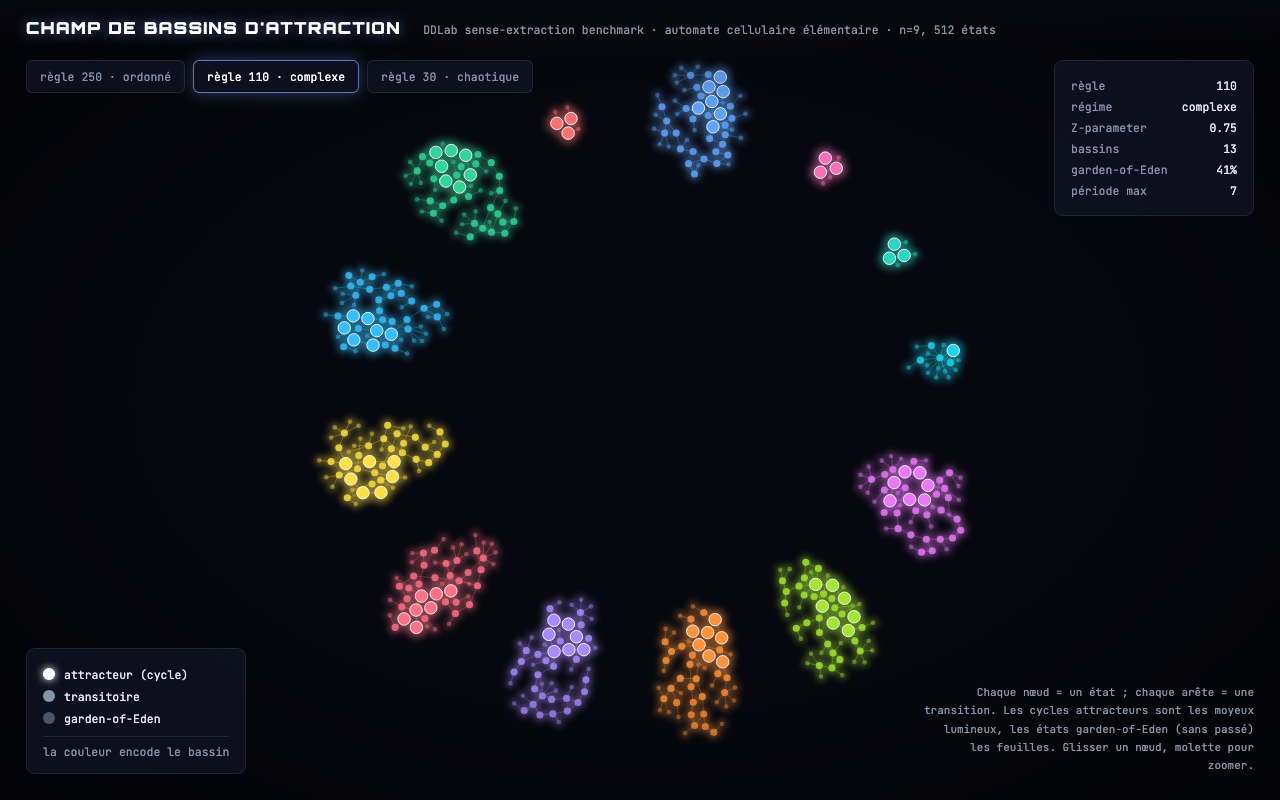
\includegraphics[width=0.80\linewidth]{figures/basin_field}
\caption{Le champ de bassins d'attraction de la règle~110 ($n{=}9$, $512$
états). Chaque sommet est un état, chaque arête une transition ; les sommets
sont colorés par bassin, les cycles attracteurs forment les moyeux lumineux et
états garden-of-Eden les feuilles ternes. Le régime complexe possède de
nombreux bassins modulaires --- la structure que le reste de l'article étudie.}
\label{fig:basin}
\end{figure}

\section{L'entraînement forward récupère la structure causale locale}
\label{sec:local}

Nous entraînons un petit GRU à prédire l'état suivant à partir de l'état
courant --- l'objectif forward (next-token). Il atteint une précision un-pas de
$1{,}0$ et généralise à des bassins retenus : il a donc appris la règle, et non
mémorisé une table.

Nous le gelons ensuite et sondons sa représentation pour des faits causaux que
l'objectif forward n'a jamais exigés : appartenance au garden-of-Eden et
in-degré. Ce sont des faits \emph{inverses} --- sur le passé d'un état, pas son
futur. Le Tableau~\ref{tab:probe} rapporte la précision en test d'une sonde
linéaire sur la règle~110, face à deux baselines : les bits d'observation
bruts, et le même réseau non entraîné.

\begin{table}[h]
\centering
\caption{Décodage par sonde linéaire de faits causaux inverses (règle 110,
$n{=}9$). L'entraînement forward rend l'appartenance au garden-of-Eden
décodable linéairement bien au-dessus des baselines observation brute et
réseau non entraîné.}
\label{tab:probe}
\begin{tabular}{lccc}
\toprule
cible & bits bruts & réseau non entraîné & entraîné forward \\
\midrule
garden-of-Eden (préc.) & 0,68 & 0,68 & \textbf{0,86} \\
in-degré (préc.)       & 0,60 & 0,60 & \textbf{0,77} \\
\bottomrule
\end{tabular}
\end{table}

L'entraînement forward construit une représentation où les faits causaux
\emph{locaux} deviennent linéairement accessibles. Deux réserves pour rester
honnête. D'abord, une sonde MLP atteint $0{,}97$ sur les bits bruts aussi : les
faits sont calculables depuis l'observation ; la représentation forward les
rend \emph{linéairement} accessibles, c'est-à-dire désintriqués. Ensuite, sur
le spectre $Z$, l'effet de désintrication est le plus marqué dans le régime
complexe ; nous le rapportons comme observation secondaire, la comparaison
étant en partie confondue avec l'équilibre des étiquettes aux extrêmes ordonné
et chaotique.

Surtout, la structure \emph{long-horizon} n'est \emph{pas} récupérée : le
partitionnement induit par la représentation forward a une information mutuelle
ajustée (AMI) quasi nulle avec la vraie partition en bassins. L'entraînement
forward récupère la structure locale et manque la structure globale --- une
distinction que la Section~\ref{sec:why} explique.

\section{La discrétisation préservant la structure existe}
\label{sec:exists}

Existe-t-il une tokenisation qui \emph{compresse} l'espace d'états tout en
\emph{préservant} la structure de bassins ? Oui, et nous l'exhibons.

Définissons le quotient par horizon $\phi_H(s) = \succf^{H}(s)$ : deux états
partagent un code si et seulement s'ils convergent vers le même état en $H$
pas. Des états qui convergent partagent un bassin, donc $\phi_H$ ne fusionne
\emph{jamais} deux bassins --- c'est, pour tout $H$, un raffinement du quotient
dynamique. À mesure que $H$ croît, les états atteignent leurs cycles
attracteurs et le nombre de codes distincts chute fortement.

\begin{table}[h]
\centering
\caption{Le quotient par horizon (règle 110, $n{=}9$, $512$ états ; sans
modèle). Il compresse alors que l'AMI avec la vraie partition en bassins reste
exactement $1{,}0$.}
\label{tab:horizon}
\begin{tabular}{rccc}
\toprule
horizon $H$ & codes distincts & taux de collision & AMI vs vrais bassins \\
\midrule
0  & 512 & 0,00 & 1,00 \\
2  & 200 & 0,61 & 1,00 \\
8  & 109 & 0,79 & 1,00 \\
16 &  73 & 0,86 & 1,00 \\
\bottomrule
\end{tabular}
\end{table}

Une discrétisation qui compresse $512$ états en $73$ tout en préservant
\emph{exactement} la structure de bassins existe donc. La question ouverte
n'est pas son existence, mais de savoir si elle peut être \emph{apprise} depuis
les observations.

\section{Les tokeniseurs appris échouent à la récupérer}
\label{sec:fail}

Nous rendons chaque état en image et entraînons un tokeniseur sur les images,
puis projetons la vraie dynamique à travers les codes appris et mesurons à quel
point le graphe de transition latent induit préserve la structure de bassins
(AMI), en fonction de la taille du codebook $K$.

Nous testons cinq objectifs : reconstruction d'image ; prédiction de l'image
suivante ; prédiction d'image multi-horizon (futur lointain) ; contrastif
temporel un-pas (InfoNCE, le successeur comme positif) ; et contrastif
temporel à futur lointain, conçu pour casser la similarité perceptuelle
locale. Le Tableau~\ref{tab:cliff} montre les deux premiers ; les variantes
contrastives ne dépassent jamais une AMI $\approx 0{,}12$ pour aucun $K$.

\begin{table}[h]
\centering
\caption{AMI vs vrais bassins pour les tokeniseurs appris (règle 110, $n{=}9$).
À $K{=}512$ la tokenisation est quasi sans perte et la structure est préservée ;
la première compression forcée ($K{=}256$) la fait s'effondrer --- une falaise,
pas une pente.}
\label{tab:cliff}
\begin{tabular}{lcc}
\toprule
objectif & AMI à $K{=}512$ & AMI à $K{=}256$ \\
\midrule
reconstruction              & 0,95 & 0,02 \\
prédiction de l'image suivante & 0,99 & 0,07 \\
\bottomrule
\end{tabular}
\end{table}

\begin{figure}[t]
\centering
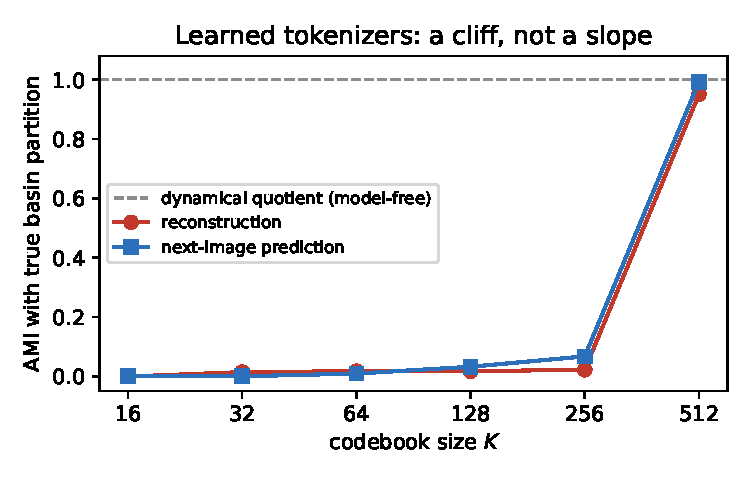
\includegraphics[width=0.64\linewidth]{figures/ami_cliff}
\caption{Préservation de la structure de bassins (AMI) en fonction de la taille
du codebook $K$, pour deux objectifs de tokeniseur appris. Les deux ne
préservent la structure que lorsque la tokenisation est quasi sans perte
($K{=}512$) ; la première compression forcée la fait s'effondrer. La ligne
pointillée marque le quotient dynamique sans modèle de la
Section~\ref{sec:exists}, qui préserve la structure exactement à tout niveau de
compression.}
\label{fig:cliff}
\end{figure}

Aucun objectif ne récupère le quotient sous compression (Figure~\ref{fig:cliff}).
Tous ne préservent la structure que lorsque la tokenisation est quasi sans
perte ; le premier bit de compression forcée la détruit. Nous avons aussi
rencontré, et documentons, les pathologies d'entraînement de ce régime ---
effondrement du codebook, et un conflit objectif/anti-effondrement --- que nous
contrôlons ; la falaise n'en est pas un artefact.

\section{Pourquoi : le désaccord perceptuel--dynamique}
\label{sec:why}

Les cinq objectifs partagent un biais inductif : ils font correspondre des
observations perceptuellement proches à des codes proches. Nous mesurons si ce
biais peut le moindrement s'aligner avec le quotient dynamique.

Pour chaque état nous prenons ses voisins perceptuels --- les états à un bit ---
et mesurons la fraction qui se trouve dans un bassin \emph{différent}. Nous
comparons ce \emph{mismatch} à la valeur attendue si les bassins étaient
assignés au hasard, à tailles identiques.

\begin{table}[h]
\centering
\caption{Désaccord perceptuel--dynamique ($n{=}9$) : fraction des voisins
perceptuels à un bit dans un bassin différent, vs une baseline d'assignation
aléatoire. Le ratio vaut $1{,}0$ dans chaque régime.}
\label{tab:mismatch}
\begin{tabular}{lcccc}
\toprule
règle & régime & mismatch & baseline aléatoire & ratio \\
\midrule
250 & ordonné   & 0,004 & 0,004 & 1,00 \\
110 & complexe  & 0,914 & 0,902 & 1,01 \\
30  & chaotique & 0,316 & 0,315 & 1,00 \\
\bottomrule
\end{tabular}
\end{table}

\begin{figure}[t]
\centering
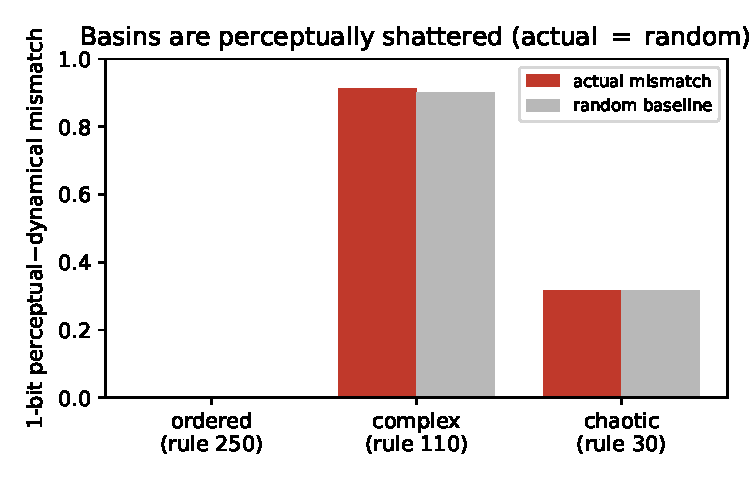
\includegraphics[width=0.64\linewidth]{figures/perceptual_mismatch}
\caption{Désaccord perceptuel--dynamique à un bit face à la baseline
d'assignation aléatoire, par régime. Les deux barres sont égales dans chaque
régime : l'appartenance à un bassin est, dans l'espace d'observation, aussi
dispersée qu'une partition aléatoire.}
\label{fig:mismatch}
\end{figure}

Le mismatch égale la baseline aléatoire. Les bassins sont \emph{perceptuellement
éclatés} : aussi dispersés dans l'espace d'observation qu'une partition
aléatoire. La proximité perceptuelle ne porte aucune information sur
l'appartenance à un bassin au-delà du taux de base.

L'échec de la Section~\ref{sec:fail} est donc \emph{structurel}. Un objectif
biaisé vers la proximité d'observation optimise une géométrie prouvablement
orthogonale au quotient dynamique --- il n'est pas sous-optimisé, il est
optimisé vers la mauvaise cible. L'image \emph{détermine} le bassin (elle
détermine l'état) ; la barrière n'est pas informationnelle mais inductive.

Cela unifie l'article. La Section~\ref{sec:local} a trouvé que l'entraînement
forward récupère la structure causale \emph{locale} ; nous trouvons ici que le
bassin est perceptuellement \emph{non-local}. Un seul biais inductif --- la
localité --- explique le succès local et l'échec global.

\section{Le contrôle positif : un objectif récursif récupère le quotient}
\label{sec:positive}

Si l'échec de la Section~\ref{sec:fail} est une propriété de l'\emph{objectif}
--- son biais de localité --- et non des données, alors un objectif qui ne
récompense pas la proximité d'observation devrait récupérer le quotient. Nous en
construisons un et le testons.

Nous entraînons un encodeur $\phi$ sur l'équation de point fixe de la métrique
de bisimulation,
\[
  d\big(\phi(x),\phi(x')\big) \;\approx\;
  \mathbb{1}[\ell(x)\neq\ell(x')] \;+\; \gamma\,
  d\big(\phi(\succf(x)),\phi(\succf(x'))\big),
\]
où $\ell$ est un observable de base grossier (la densité de l'état), $\gamma<1$
rend la récursion contractante, et la cible du terme récursif est lue sur une
copie de $\phi$ mise à jour lentement. L'objectif ne fait jamais référence à la
proximité d'observation au-delà de $\ell$ : il vit entièrement sur le graphe de
transition. Nous scorons le plongement ($k$-moyennes, puis AMI) face au quotient
de bisimulation exact relatif à $\ell$.

\begin{table}[h]
\centering
\caption{AMI avec le quotient de bisimulation exact ($n{=}10$). Un objectif
récursif sur la dynamique récupère le quotient que la baseline perceptuelle
manque ; c'est le terme récursif lui-même --- non l'observable de base --- qui
fait le travail.}
\label{tab:positive}
\begin{tabular}{lccc}
\toprule
objectif & règle 250 & règle 110 & règle 30 \\
         & (ordonné) & (complexe) & (chaotique) \\
\midrule
bits bruts (perceptuel)                & 0,10 & 0,01 & 0,01 \\
observable de base seul ($\gamma{=}0$) & 0,60 & 0,26 & 0,19 \\
récursif ($\gamma{=}0{,}5$)            & \textbf{0,95} & \textbf{0,70} & \textbf{0,52} \\
\bottomrule
\end{tabular}
\end{table}

L'objectif récursif récupère le quotient dans chaque régime
(Tableau~\ref{tab:positive}) : AMI $0{,}95/0{,}70/0{,}52$, contre
$\le 0{,}10$ pour la baseline observation brute. C'est la récursion qui compte
--- l'observable de base seul ($\gamma{=}0$) n'atteint que
$0{,}60/0{,}26/0{,}19$ ; ajouter le terme récursif des « futurs des futurs »
double à peu près la récupération. La difficulté suit le régime : le quotient
ordonné est petit et presque parfaitement récupéré, le quotient chaotique a de
nombreux blocs et n'est récupéré qu'en partie.

La barrière des Sections~\ref{sec:fail}--\ref{sec:why} est donc réelle mais
\emph{propre à l'objectif} : une propriété des objectifs de proximité
d'observation, qui se dissout pour un objectif défini sur la dynamique. Une
réserve honnête : le quotient de bisimulation est plus fin que la partition en
bassins --- il distingue la phase transitoire, que le bassin ignore --- de sorte
que récupérer les \emph{bassins} en propre est une cible distincte, plus dure.
Une variante d'invariance ($\phi(x)\approx\phi(\succf(x))$, l'objectif de
Koopman à valeur propre un) récupère les bassins dans le régime ordonné
(AMI $0{,}48$ contre $0{,}00$ pour la baseline perceptuelle) mais se dégrade
vers le chaos, confondue par le déséquilibre des tailles de bassins ; nous le
rapportons comme résultat secondaire.

\section{Discussion et limites}

\paragraph{Implications.}
On ne devrait pas supposer que les latents de reconstruction ou de contrastif
d'instance portent la structure causale-dynamique ; là où la structure cible
est non-locale dans l'espace d'observation, un objectif à biais de localité lui
est structurellement inadapté. La Section~\ref{sec:positive} le confirme : un
objectif défini récursivement sur la dynamique, plutôt que sur la proximité
d'observation, récupère le quotient que tout objectif perceptuel manque.
La mesure de mismatch de la
Section~\ref{sec:why} est un test \emph{a priori} bon marché : si une structure
cible est perceptuellement éclatée par rapport à l'observation, un objectif
perceptuel échouera avant tout entraînement. Plus largement, le banc d'essai
lui-même est une méthodologie utilisable --- auditer un apprenant de
représentations sur un petit système énumérable où la réponse causale est
connue.

\paragraph{Limites.}
Les systèmes sont petits ($n \le 14$ dans les expériences). C'est délibéré : une
vérité-terrain exacte et sans échantillonnage exige un espace d'états
énumérable. Le banc d'essai est un audit contrôlé, pas une affirmation sur un
grand modèle spécifique ; le transfert du mécanisme aux grands world models
continus à latents appris est la question suivante naturelle et n'est pas
établi ici. Plusieurs résultats utilisent des instances uniques ; le négatif
central (le ratio de mismatch perceptuel) est robuste à travers les régimes,
mais une moyenne d'ensemble renforcerait les observations secondaires.
L'objectif récursif de la Section~\ref{sec:positive} est montré à
$\gamma{=}0{,}5$ ; la limite $\gamma\to1$ et la variante d'invariance visant
les bassins sont moins stables et rapportées comme secondaires.

\section{Conclusion}

Sur des systèmes dynamiques discrets à vérité-terrain exacte, une discrétisation
compressée et préservant la structure de l'espace d'états existe prouvablement
--- le quotient dynamique --- et cinq objectifs d'apprentissage de
représentations standards échouent prouvablement à la récupérer depuis les
observations. La raison est structurelle : le quotient est perceptuellement
éclaté, et les objectifs biaisés vers la proximité d'observation optimisent une
géométrie orthogonale. Un objectif défini au contraire sur la dynamique --- une
métrique de bisimulation récursive --- le récupère, situant l'échec dans
l'objectif et non dans les données. La perception n'est pas la causalité ; un
objectif qui poursuit la première ne trouvera pas la seconde, mais un objectif
défini sur la dynamique, si.

\paragraph{Reproductibilité.}
Toutes les expériences sont exactes ou seedées ; l'implémentation (le banc
d'essai, les scripts d'expérience et une suite de tests) est publiée.

\bibliographystyle{plainnat}
\bibliography{references}

\end{document}
